% Options for packages loaded elsewhere
\PassOptionsToPackage{unicode}{hyperref}
\PassOptionsToPackage{hyphens}{url}
%
\documentclass[
  ignorenonframetext,
]{beamer}
\usepackage{pgfpages}
\setbeamertemplate{caption}[numbered]
\setbeamertemplate{caption label separator}{: }
\setbeamercolor{caption name}{fg=normal text.fg}
\beamertemplatenavigationsymbolsempty
% Prevent slide breaks in the middle of a paragraph
\widowpenalties 1 10000
\raggedbottom
\setbeamertemplate{part page}{
  \centering
  \begin{beamercolorbox}[sep=16pt,center]{part title}
    \usebeamerfont{part title}\insertpart\par
  \end{beamercolorbox}
}
\setbeamertemplate{section page}{
  \centering
  \begin{beamercolorbox}[sep=12pt,center]{part title}
    \usebeamerfont{section title}\insertsection\par
  \end{beamercolorbox}
}
\setbeamertemplate{subsection page}{
  \centering
  \begin{beamercolorbox}[sep=8pt,center]{part title}
    \usebeamerfont{subsection title}\insertsubsection\par
  \end{beamercolorbox}
}
\AtBeginPart{
  \frame{\partpage}
}
\AtBeginSection{
  \ifbibliography
  \else
    \frame{\sectionpage}
  \fi
}
\AtBeginSubsection{
  \frame{\subsectionpage}
}

\usepackage{amsmath,amssymb}
\usepackage{iftex}
\ifPDFTeX
  \usepackage[T1]{fontenc}
  \usepackage[utf8]{inputenc}
  \usepackage{textcomp} % provide euro and other symbols
\else % if luatex or xetex
  \usepackage{unicode-math}
  \defaultfontfeatures{Scale=MatchLowercase}
  \defaultfontfeatures[\rmfamily]{Ligatures=TeX,Scale=1}
\fi
\usepackage{lmodern}
\usecolortheme{Flip}
\usefonttheme{serif} % use mainfont rather than sansfont for slide text
\useinnertheme{Flip}
\useoutertheme{Flip}
\ifPDFTeX\else  
    % xetex/luatex font selection
  \setmainfont[]{VisbyCF-Medium}
  \setsansfont[]{Latin Modern Sans}
  \setmathfont[]{Latin Modern Math}
\fi
% Use upquote if available, for straight quotes in verbatim environments
\IfFileExists{upquote.sty}{\usepackage{upquote}}{}
\IfFileExists{microtype.sty}{% use microtype if available
  \usepackage[]{microtype}
  \UseMicrotypeSet[protrusion]{basicmath} % disable protrusion for tt fonts
}{}
\makeatletter
\@ifundefined{KOMAClassName}{% if non-KOMA class
  \IfFileExists{parskip.sty}{%
    \usepackage{parskip}
  }{% else
    \setlength{\parindent}{0pt}
    \setlength{\parskip}{6pt plus 2pt minus 1pt}}
}{% if KOMA class
  \KOMAoptions{parskip=half}}
\makeatother
\usepackage{xcolor}
\newif\ifbibliography
\setlength{\emergencystretch}{3em} % prevent overfull lines
\setcounter{secnumdepth}{-\maxdimen} % remove section numbering

\usepackage{color}
\usepackage{fancyvrb}
\newcommand{\VerbBar}{|}
\newcommand{\VERB}{\Verb[commandchars=\\\{\}]}
\DefineVerbatimEnvironment{Highlighting}{Verbatim}{commandchars=\\\{\}}
% Add ',fontsize=\small' for more characters per line
\usepackage{framed}
\definecolor{shadecolor}{RGB}{241,243,245}
\newenvironment{Shaded}{\begin{snugshade}}{\end{snugshade}}
\newcommand{\AlertTok}[1]{\textcolor[rgb]{0.68,0.00,0.00}{#1}}
\newcommand{\AnnotationTok}[1]{\textcolor[rgb]{0.37,0.37,0.37}{#1}}
\newcommand{\AttributeTok}[1]{\textcolor[rgb]{0.40,0.45,0.13}{#1}}
\newcommand{\BaseNTok}[1]{\textcolor[rgb]{0.68,0.00,0.00}{#1}}
\newcommand{\BuiltInTok}[1]{\textcolor[rgb]{0.00,0.23,0.31}{#1}}
\newcommand{\CharTok}[1]{\textcolor[rgb]{0.13,0.47,0.30}{#1}}
\newcommand{\CommentTok}[1]{\textcolor[rgb]{0.37,0.37,0.37}{#1}}
\newcommand{\CommentVarTok}[1]{\textcolor[rgb]{0.37,0.37,0.37}{\textit{#1}}}
\newcommand{\ConstantTok}[1]{\textcolor[rgb]{0.56,0.35,0.01}{#1}}
\newcommand{\ControlFlowTok}[1]{\textcolor[rgb]{0.00,0.23,0.31}{#1}}
\newcommand{\DataTypeTok}[1]{\textcolor[rgb]{0.68,0.00,0.00}{#1}}
\newcommand{\DecValTok}[1]{\textcolor[rgb]{0.68,0.00,0.00}{#1}}
\newcommand{\DocumentationTok}[1]{\textcolor[rgb]{0.37,0.37,0.37}{\textit{#1}}}
\newcommand{\ErrorTok}[1]{\textcolor[rgb]{0.68,0.00,0.00}{#1}}
\newcommand{\ExtensionTok}[1]{\textcolor[rgb]{0.00,0.23,0.31}{#1}}
\newcommand{\FloatTok}[1]{\textcolor[rgb]{0.68,0.00,0.00}{#1}}
\newcommand{\FunctionTok}[1]{\textcolor[rgb]{0.28,0.35,0.67}{#1}}
\newcommand{\ImportTok}[1]{\textcolor[rgb]{0.00,0.46,0.62}{#1}}
\newcommand{\InformationTok}[1]{\textcolor[rgb]{0.37,0.37,0.37}{#1}}
\newcommand{\KeywordTok}[1]{\textcolor[rgb]{0.00,0.23,0.31}{#1}}
\newcommand{\NormalTok}[1]{\textcolor[rgb]{0.00,0.23,0.31}{#1}}
\newcommand{\OperatorTok}[1]{\textcolor[rgb]{0.37,0.37,0.37}{#1}}
\newcommand{\OtherTok}[1]{\textcolor[rgb]{0.00,0.23,0.31}{#1}}
\newcommand{\PreprocessorTok}[1]{\textcolor[rgb]{0.68,0.00,0.00}{#1}}
\newcommand{\RegionMarkerTok}[1]{\textcolor[rgb]{0.00,0.23,0.31}{#1}}
\newcommand{\SpecialCharTok}[1]{\textcolor[rgb]{0.37,0.37,0.37}{#1}}
\newcommand{\SpecialStringTok}[1]{\textcolor[rgb]{0.13,0.47,0.30}{#1}}
\newcommand{\StringTok}[1]{\textcolor[rgb]{0.13,0.47,0.30}{#1}}
\newcommand{\VariableTok}[1]{\textcolor[rgb]{0.07,0.07,0.07}{#1}}
\newcommand{\VerbatimStringTok}[1]{\textcolor[rgb]{0.13,0.47,0.30}{#1}}
\newcommand{\WarningTok}[1]{\textcolor[rgb]{0.37,0.37,0.37}{\textit{#1}}}

\providecommand{\tightlist}{%
  \setlength{\itemsep}{0pt}\setlength{\parskip}{0pt}}\usepackage{longtable,booktabs,array}
\usepackage{calc} % for calculating minipage widths
\usepackage{caption}
% Make caption package work with longtable
\makeatletter
\def\fnum@table{\tablename~\thetable}
\makeatother
\usepackage{graphicx}
\makeatletter
\def\maxwidth{\ifdim\Gin@nat@width>\linewidth\linewidth\else\Gin@nat@width\fi}
\def\maxheight{\ifdim\Gin@nat@height>\textheight\textheight\else\Gin@nat@height\fi}
\makeatother
% Scale images if necessary, so that they will not overflow the page
% margins by default, and it is still possible to overwrite the defaults
% using explicit options in \includegraphics[width, height, ...]{}
\setkeys{Gin}{width=\maxwidth,height=\maxheight,keepaspectratio}
% Set default figure placement to htbp
\makeatletter
\def\fps@figure{htbp}
\makeatother

\usepackage{booktabs}
\usepackage{longtable}
\usepackage{array}
\usepackage{multirow}
\usepackage{wrapfig}
\usepackage{float}
\usepackage{colortbl}
\usepackage{pdflscape}
\usepackage{tabu}
\usepackage{threeparttable}
\usepackage{threeparttablex}
\usepackage[normalem]{ulem}
\usepackage{makecell}
\usepackage{xcolor}
\usepackage{tabu}
\usepackage{mathtools}
\usepackage{mathrsfs}
\makeatletter
\makeatother
\makeatletter
\makeatother
\makeatletter
\@ifpackageloaded{caption}{}{\usepackage{caption}}
\AtBeginDocument{%
\ifdefined\contentsname
  \renewcommand*\contentsname{Table of contents}
\else
  \newcommand\contentsname{Table of contents}
\fi
\ifdefined\listfigurename
  \renewcommand*\listfigurename{List of Figures}
\else
  \newcommand\listfigurename{List of Figures}
\fi
\ifdefined\listtablename
  \renewcommand*\listtablename{List of Tables}
\else
  \newcommand\listtablename{List of Tables}
\fi
\ifdefined\figurename
  \renewcommand*\figurename{Figure}
\else
  \newcommand\figurename{Figure}
\fi
\ifdefined\tablename
  \renewcommand*\tablename{Table}
\else
  \newcommand\tablename{Table}
\fi
}
\@ifpackageloaded{float}{}{\usepackage{float}}
\floatstyle{ruled}
\@ifundefined{c@chapter}{\newfloat{codelisting}{h}{lop}}{\newfloat{codelisting}{h}{lop}[chapter]}
\floatname{codelisting}{Listing}
\newcommand*\listoflistings{\listof{codelisting}{List of Listings}}
\makeatother
\makeatletter
\@ifpackageloaded{caption}{}{\usepackage{caption}}
\@ifpackageloaded{subcaption}{}{\usepackage{subcaption}}
\makeatother
\makeatletter
\@ifpackageloaded{tcolorbox}{}{\usepackage[skins,breakable]{tcolorbox}}
\makeatother
\makeatletter
\@ifundefined{shadecolor}{\definecolor{shadecolor}{rgb}{.97, .97, .97}}
\makeatother
\makeatletter
\makeatother
\makeatletter
\makeatother
\ifLuaTeX
  \usepackage{selnolig}  % disable illegal ligatures
\fi
\IfFileExists{bookmark.sty}{\usepackage{bookmark}}{\usepackage{hyperref}}
\IfFileExists{xurl.sty}{\usepackage{xurl}}{} % add URL line breaks if available
\urlstyle{same} % disable monospaced font for URLs
\hypersetup{
  pdftitle={Analyse de survie},
  pdfauthor={Léo Belzile},
  hidelinks,
  pdfcreator={LaTeX via pandoc}}

\title{Analyse de survie}
\subtitle{Analyse multidimensionnelle appliquée}
\author{Léo Belzile}
\date{}
\institute{HEC Montréal}

\begin{document}
\frame{\titlepage}
\ifdefined\Shaded\renewenvironment{Shaded}{\begin{tcolorbox}[frame hidden, interior hidden, enhanced, borderline west={3pt}{0pt}{shadecolor}, boxrule=0pt, sharp corners, breakable]}{\end{tcolorbox}}\fi

\begin{frame}{Analyse de survie}
\protect\hypertarget{analyse-de-survie}{}
Étude du temps avant qu'un événement survienne.

\begin{itemize}
\tightlist
\item
  temps qu'un client demeure abonné à un service offert par notre
  compagnie.
\item
  ancienneté d'un travailleur au service d'une compagnie.
\item
  durée de vie d'une franchise ou avant la faillite d'une entreprise.
\item
  temps avant le prochain achat d'un(e) client(e).
\item
  temps durant lequel une personne est au chômage.
\end{itemize}
\end{frame}

\begin{frame}{Mécanismes de survie}
\protect\hypertarget{muxe9canismes-de-survie}{}
La survie est caractérisée par la présence d'information
\textbf{partielle}.

Les données sont sujettes à \textbf{troncature} et à \textbf{censure}.
\end{frame}

\begin{frame}{Définition de la censure}
\protect\hypertarget{duxe9finition-de-la-censure}{}
Le temps réel de l'événement n'est pas observé (information partielle).

\begin{itemize}
\tightlist
\item
  Censure à droite: l'événement n'est pas encore survenu au temps \(t\):
  on sait que \(T > t\).
\item
  Censure à gauche: l'événement survient avant le temps \(t\), donc la
  vraie valeur est inférieure à la valeur observée (\(T < t\))
\item
  Censure par intervalle: l'événement est survenu dans la plage
  \([t_1, t_2]\) (données arrondies)
\end{itemize}
\end{frame}

\begin{frame}{Définitions de la troncature}
\protect\hypertarget{duxe9finitions-de-la-troncature}{}
La plage des valeurs possibles est tronquée.

\begin{itemize}
\tightlist
\item
  troncature à gauche: le temps minimum est supérieur à \(t_0\)
\item
  troncature à droite: le temps maximum est inférieur à \(t_1\)
\item
  troncature par intervalle: le temps de l'événement doit survenir entre
  \(t_0\) et \(t_1\).
\end{itemize}
\end{frame}

\begin{frame}{Exemple: étude sur le chômage}
\protect\hypertarget{exemple-uxe9tude-sur-le-chuxf4mage}{}
\begin{itemize}
\tightlist
\item
  Certaines personnes seront déjà au chômage au début de l'étude
  (troncature à gauche): le temps réel sera supérieur à la durée écoulée
\item
  Certaines personnes ont trouvé un emploi entre deux prises de contact,
  mais la date exacte est inconnue (censure par intervalle).
\item
  D'autres personnes seront toujours au chômage à la fin de l'étude
  (censure à droite).
\end{itemize}
\end{frame}

\begin{frame}{Diagramme de Lexis}
\protect\hypertarget{diagramme-de-lexis}{}
\begin{columns}[T]
\begin{column}{0.5\textwidth}
\begin{figure}

{\centering 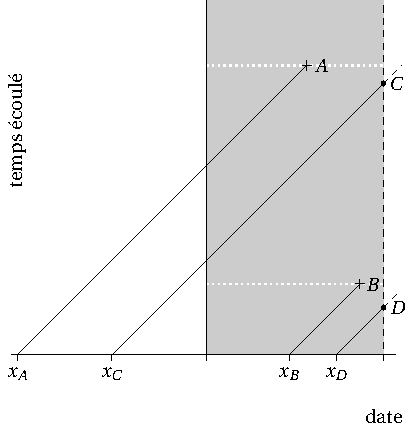
\includegraphics{figures/Lexis_censure.pdf}

}

\caption{Diagramme de Lexis pour données tronquées à gauche (\(A\) et
\(C\)) et censurées à droite (\(C\) et \(D\)).}

\end{figure}
\end{column}

\begin{column}{0.4\textwidth}
\begin{itemize}
\tightlist
\item
  On trace une droite de pente 1 représentant la durée en fonction du
  temps (date au calendrier).
\item
  La fenêtre définit la période de collecte de donnée.
\item
  On peut lire le temps initial et le temps final sur l'axe des \(y\).
\item
  La censure est indiquée par des cercles, les événements par des croix.
\end{itemize}
\end{column}
\end{columns}
\end{frame}

\begin{frame}{Troncature par intervalle}
\protect\hypertarget{troncature-par-intervalle}{}
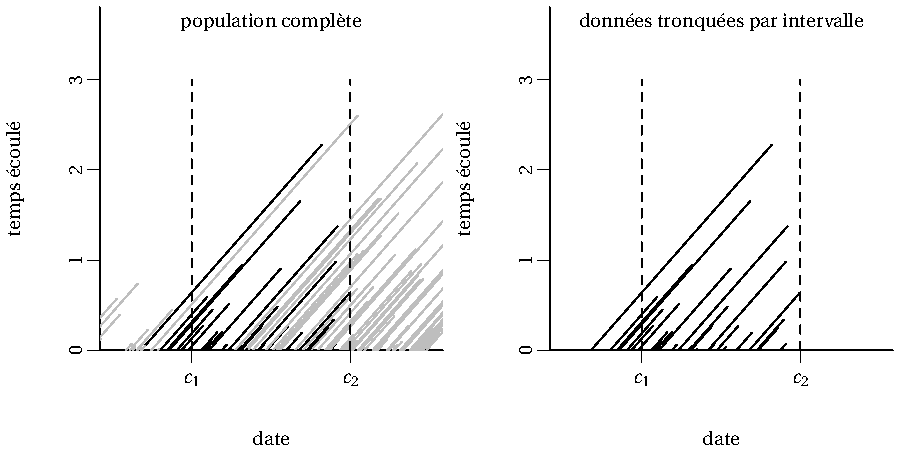
\includegraphics{figures/lexis_troncationintervalle.pdf}

\footnotesize

On s'intéresse à la durée de la relation d'emploi: seules les personnes
à l'emploi qui ont pris leur retraite entre 2009 et 2021 sont
considérées pour l'étude.
\end{frame}

\begin{frame}{Exemple de données de survie}
\protect\hypertarget{exemple-de-donnuxe9es-de-survie}{}
Tableau extrait de \href{https://doi.org/10.1093/gerona/glv113}{Hanamaya
et Sibuya (2016)}

\begin{figure}

{\centering 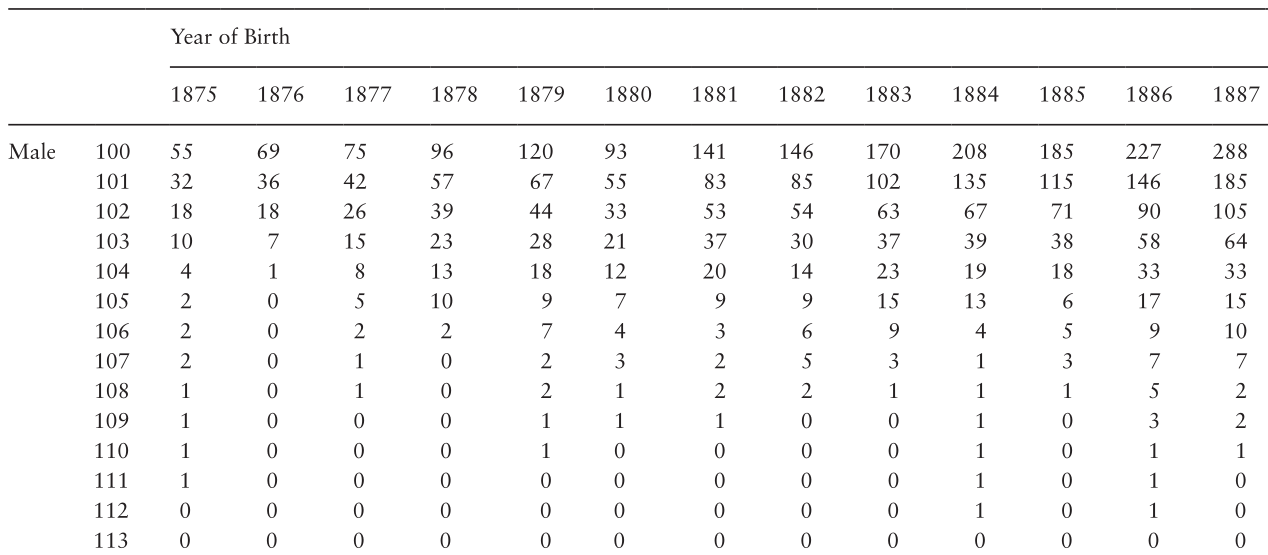
\includegraphics[width=0.8\textwidth,height=\textheight]{figures/Sibuya_tabular.png}

}

\caption{Âge au décès (cohortes éteintes) de centenaires Japonais.}

\end{figure}

\small

Données censurées par intervalles et tronquées à droite (l'âge maximum
des personnes en date de collecte des données en 2012).

\normalsize
\end{frame}

\begin{frame}{Censure informative ou pas?}
\protect\hypertarget{censure-informative-ou-pas}{}
La censure peut être aléatoire ou non-informative:

\begin{itemize}
\tightlist
\item
  une étude finit en juin (censure administrative)
\item
  une personne déménage dans une autre province et n'est plus suivie
\end{itemize}

Si la censure est informative, les outils présentés ne sont pas
adéquats!

\begin{itemize}
\tightlist
\item
  un patient d'une étude clinique est déchargé d'un protocole médical
  car il est trop mal en point.
\end{itemize}
\end{frame}

\begin{frame}{Exemple}
\protect\hypertarget{exemple}{}
Où est l'erreur de logique dans l'analyse suivante?

\begin{figure}

{\centering 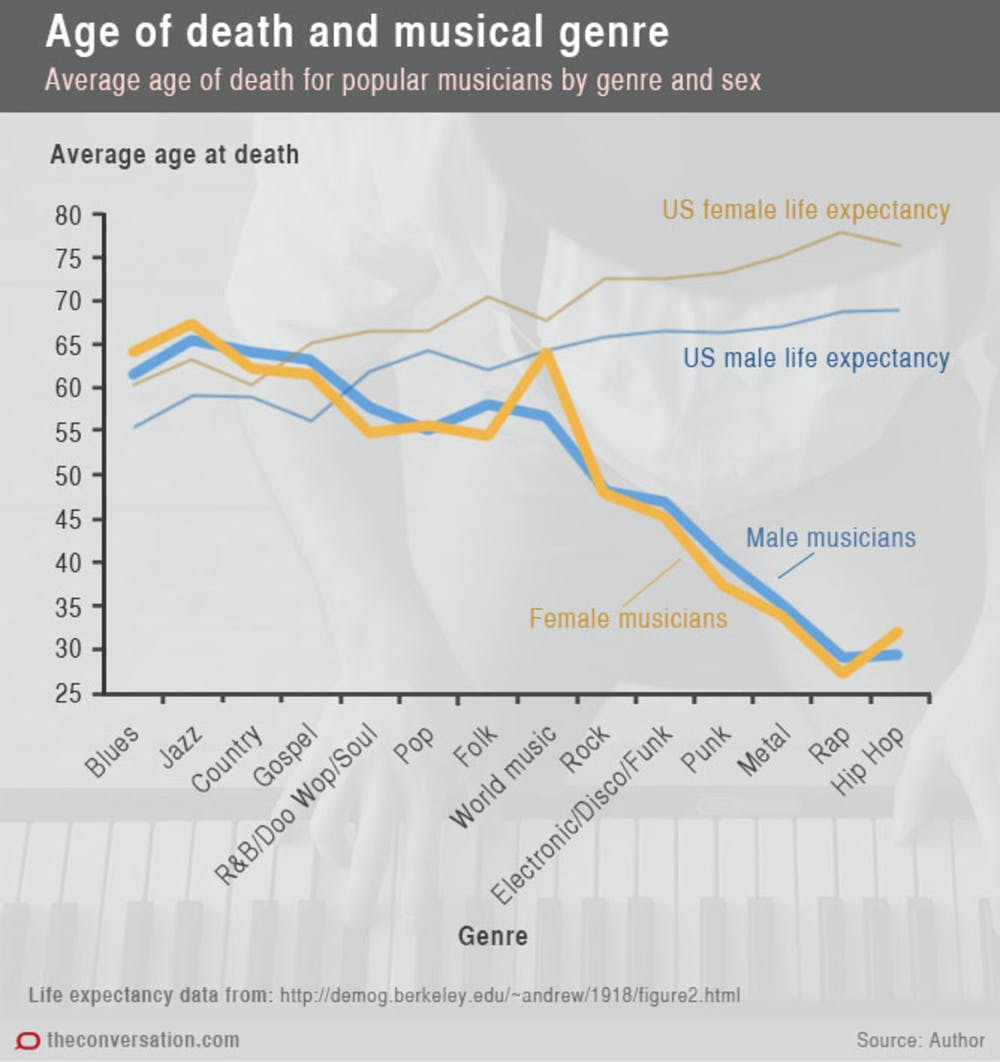
\includegraphics[width=0.6\textwidth,height=\textheight]{figures/rightcensoring_illustration-age_death_music_genre.jpg}

}

\end{figure}
\end{frame}

\begin{frame}{Contenu du cours}
\protect\hypertarget{contenu-du-cours}{}
La survie est un sujet très compliqué\ldots{}

On s'intéressera uniquement à la censure à droite (non informative).

Le cours ne couvrira que des méthodes nonparamétriques ou
semiparamétriques.
\end{frame}

\begin{frame}{Données}
\protect\hypertarget{donnuxe9es}{}
La structure de données de base que l'on doit avoir pour travailler est
la suivante:

\begin{enumerate}
\tightlist
\item
  une variable temps, \(T\).
\item
  une variable binaire \(C\) (censure).
\item
  des variables explicatives \(X_1, \ldots, X_p\)
\end{enumerate}

On considère l'exemple d'une entreprise de télécommunications qui veut
connaître les facteurs influençant la durée d'abonnement à son service
de téléphone cellulaire.
\end{frame}

\begin{frame}[fragile]{Temps d'abonnement à un forfait cellulaire}
\protect\hypertarget{temps-dabonnement-uxe0-un-forfait-cellulaire}{}
Les données \texttt{survie1} contiennent les variables suivantes.

\begin{itemize}
\tightlist
\item
  \(\texttt{temps}\): temps (en semaines) que le client est resté abonné
  au service de téléphone cellulaire. Il s'agit du vrai temps si le
  client n'est plus abonné et d'une borne inférieure si le client est
  toujours abonné.
\item
  \texttt{censure}: variable binaire qui indique si la variable
  \texttt{t} est censurée (\texttt{0} si le client est toujours abonné)
  ou non (\texttt{1}, la variable \texttt{t} est la durée finale de
  l'abonnement).
\item
  \texttt{age}: âge du client au début de l'abonnement.
\item
  \texttt{sexe}: sexe du client, soit femme (\texttt{1}), soit homme
  (\texttt{0}).
\item
  \texttt{service}: nombre de services en plus du cellulaire auquel le
  client est abonné parmi internet, téléphone fixe, télévision (câble ou
  antenne parabolique).
\item
  \texttt{region}: région où habite le client en ce moment (valeurs
  entre \texttt{1} et \texttt{5}).
\end{itemize}
\end{frame}

\begin{frame}{Fonction de survie}
\protect\hypertarget{fonction-de-survie}{}
Soit \(F(t)=\Pr(T \leq t)\) la fonction de répartition du temps de
survie \(t\). La fonction de survie, \begin{align*}
S(t)= \Pr(T > t) = 1-F(t),
\end{align*} donne la probabilité que le temps de survie soit supérieur
à \(t\).
\end{frame}

\begin{frame}{Estimateur de Kaplan--Meier}
\protect\hypertarget{estimateur-de-kaplanmeier}{}
L'estimateur de Kaplan--Meier est un estimateur de la fonction de survie
en présense de censure à droite.

Cette méthode est nonparamétrique en ce sens qu'on ne suppose aucun
modèle et qu'on suppose uniquement que la censure est non-informative.
\end{frame}

\begin{frame}[fragile]{Kaplan--Meier avec \textbf{R}}
\protect\hypertarget{kaplanmeier-avec-r}{}
\begin{Shaded}
\begin{Highlighting}[numbers=left,,]
\FunctionTok{library}\NormalTok{(survival)}
\FunctionTok{data}\NormalTok{(survie1, }\AttributeTok{package =} \StringTok{"hecmulti"}\NormalTok{)}
\CommentTok{\# Estimateur de Kaplan{-}Meier}
\CommentTok{\# La réponse "temps" est le temps de survie }
\CommentTok{\# et l\textquotesingle{}indicateur de censure "censure" est}
\CommentTok{\# "0" pour censuré à droite, "1" pour événement}
\NormalTok{kapm }\OtherTok{\textless{}{-}} \FunctionTok{survfit}\NormalTok{(}
  \FunctionTok{Surv}\NormalTok{(temps, censure) }\SpecialCharTok{\textasciitilde{}} \DecValTok{1}\NormalTok{, }
  \CommentTok{\#\textasciitilde{}1 =\textgreater{} aucune variable explicative}
  \AttributeTok{type =} \StringTok{"kaplan{-}meier"}\NormalTok{, }
  \AttributeTok{conf.type =} \StringTok{"log"}\NormalTok{, }\CommentTok{\#type d\textquotesingle{}intervalle de conf.}
  \AttributeTok{data =}\NormalTok{ survie1)}
\end{Highlighting}
\end{Shaded}
\end{frame}

\begin{frame}[fragile]{Méthodes pour \texttt{survfit}}
\protect\hypertarget{muxe9thodes-pour-survfit}{}
\begin{Shaded}
\begin{Highlighting}[numbers=left,,]
\CommentTok{\# Tableau résumé de la survie}
\FunctionTok{summary}\NormalTok{(kapm)  }
\CommentTok{\# Graphique de la fonction de survie}
\FunctionTok{plot}\NormalTok{(kapm) }\CommentTok{\# graphique de base}
\CommentTok{\# Quantiles (par défaut, quartiles)}
\FunctionTok{quantile}\NormalTok{(kapm)}
\end{Highlighting}
\end{Shaded}

Parmi les 500 observations, il y a

\begin{itemize}
\tightlist
\item
  334 clients qui ont terminé leur abonnement et
\item
  166 qui sont censurées à droite.
\end{itemize}

La fonction résumé (\texttt{summary}) renvoit l'estimation de la
fonction de survie pour chaque temps d'échec (événement).

\begin{itemize}
\tightlist
\item
  l'estimateur est \emph{indéfini} à ces valeurs.
\end{itemize}
\end{frame}

\begin{frame}{Tableau résumé (sortie tronqué)}
\protect\hypertarget{tableau-ruxe9sumuxe9-sortie-tronquuxe9}{}
\hypertarget{tbl-survie1-tableau}{}
\begin{table}
\caption{\label{tbl-survie1-tableau}Estimation de la fonction de survie (Kaplan--Meier) pour les données de
survie d'abonnement. }\tabularnewline

\centering
\resizebox{\linewidth}{!}{
\begin{tabular}{rrrrrr}
\toprule
temps & nb à risque & nb échecs & nb cumul. & survie & erreur-type\\
\midrule
2 & 500 & 1 & 1 & 0.9980 & 0.002\\
11 & 499 & 1 & 2 & 0.9960 & 0.003\\
14 & 498 & 1 & 3 & 0.9940 & 0.003\\
18 & 497 & 1 & 4 & 0.9920 & 0.004\\
27 & 496 & 1 & 5 & 0.9900 & 0.004\\
29 & 495 & 1 & 6 & 0.9880 & 0.005\\
30 & 494 & 1 & 7 & 0.9860 & 0.005\\
34 & 493 & 4 & 11 & 0.9780 & 0.007\\
 &  &  &  &  & \\
189 & 13 & 1 & 331 & 0.2037 & 0.028\\
202 & 6 & 1 & 332 & 0.1697 & 0.039\\
216 & 2 & 2 & 334 & 0.0000 & \\
\bottomrule
\end{tabular}}
\end{table}
\end{frame}

\begin{frame}{Calcul du temps de survie}
\protect\hypertarget{calcul-du-temps-de-survie}{}
La fonction de survie estimée est une fonction escalier.

Pour trouver la survie au temps \(t\), on regarde la valeur rapportée
dans le tableau pour le temps \(t_0 \leq t\) le plus proche.

La survie, soit la probabilité estimée que le temps d'abonnement dépasse

\begin{itemize}
\tightlist
\item
  30 semaines, est 0.986;
\item
  32 semaines, est 0.986.
\end{itemize}
\end{frame}

\begin{frame}{Graphique de la fonction de survie}
\protect\hypertarget{graphique-de-la-fonction-de-survie}{}
\begin{figure}

{\centering \includegraphics[width=0.85\textwidth,height=\textheight]{MATH60602-diapos8_files/figure-beamer/fig-km-survie1-1.pdf}

}

\caption{\label{fig-km-survie1}Estimation de Kaplan--Meier de la
fonction de survie pour les données d'abonnement avec intervalles de
confiance ponctuels à 95\%.}

\end{figure}
\end{frame}

\begin{frame}[fragile]{Comprendre l'estimateur de Kaplan--Meier}
\protect\hypertarget{comprendre-lestimateur-de-kaplanmeier}{}
\begin{itemize}
\tightlist
\item
  On parle d'\textbf{échec} au temps \(t_i\) si \(T = t_i\) et \(C=0\)
  (événement observé au temps \(t_i\)).
\item
  Le nombre de \textbf{personnes à risque} au temps \(t_i\) est le total
  des observations dont le temps mesuré excède \(t_i\) (censure et
  événements postérieurs à \(t_i\) si troncation à gauche)
\end{itemize}

\textbf{Construction}:

\begin{itemize}
\tightlist
\item
  Ordonner les temps (uniques) où il y a des échecs (temps où
  \texttt{censure\ =\ 1}), disons \(t_{(1)} \leq \cdots \leq t_{(m)}\)
\item
  À chaque temps \(t_{(i)}\) \((i=1, \ldots m)\), on calcule le nombre
  de personnes à risque, \(r_i\), et le nombre d'échecs, \(d_i\).
\item
  Le risque empirique est \(\widehat{h}_i = r_i/d_i\), la proportion
  d'échecs parmi les personnes à risque.
\end{itemize}
\end{frame}

\begin{frame}{Dérivation de Kaplan--Meier}
\protect\hypertarget{duxe9rivation-de-kaplanmeier}{}
L'estimateur de Kaplan--Meier définit une \textbf{fonction escalier}
\footnotesize

\begin{itemize}
\tightlist
\item
  Entre \(t=0\) et \(t=t_{(1)}\), la survie est de 1.
\item
  Entre \(t=t_{(1)}\) et \(t=t_{(2)}\), la survie est
  \(1-\widehat{h}_1\).
\item
  Entre \(t=t_{(2)}\) et \(t=t_{(3)}\), la survie est
  \((1-\widehat{h}_1) \times (1-\widehat{h}_2)\).
\end{itemize}

\normalsize

Pour un temps \(t\) donné, on multiplie tous les termes
(\(1-\widehat{h}_i\)) des temps d'échecs passés, \begin{align*}
 \widehat{S}(t) = \prod_{i: t_{(i)} < t} \left( 1- \widehat{h}_i\right).
\end{align*}

\begin{itemize}
\tightlist
\item
  la survie ne change qu'aux valeurs de \(t_{(i)}\) (\(i=1, \ldots, m\))
\item
  les contre-marches interviennent uniquement aux temps observés
  d'\textbf{échecs}.
\item
  si la plus grande observation est censurée, la courbe de survie
  n'atteindra jamais zéro.
\end{itemize}
\end{frame}

\begin{frame}[fragile]{Syntaxe pour variable réponse}
\protect\hypertarget{syntaxe-pour-variable-ruxe9ponse}{}
La troncature à gauche impacte seulement l'ensemble des observations à
risque

\begin{itemize}
\tightlist
\item
  une personne n'est pas à risque d'échec avant le temps enregistré pour
  la censure à gauche.
\end{itemize}

Avec \texttt{survival}, la syntaxe pour la variable réponse devient
\texttt{Surv(time,\ time2,\ event,\ type\ =\ \textquotesingle{}right\textquotesingle{})},
où

\begin{itemize}
\tightlist
\item
  \texttt{time} est le temps de troncature à gauche, ou zéro
\item
  \texttt{time2} est le temps de défaillance, ou de censure à droite
\item
  \texttt{event} est une variable entière qui vaut 1 pour les temps
  observés et 0 pour les temps censurés à droite.
\end{itemize}
\end{frame}

\begin{frame}{Quantiles de la fonction de survie}
\protect\hypertarget{quantiles-de-la-fonction-de-survie}{}
On obtient le quantile à partir du tableau: c'est le premier temps
d'échec où la survie est inférieure au quantile (la ligne horizontale au
quantile traverse une contre-marche).

\begin{table}
\centering
\begin{tabular}{rrrr}
\toprule
niveau (\%) & quantile & IC 95\% (borne inf.) & IC 95\% (borne sup.)\\
\midrule
25 & 84 & 80 & 90\\
50 & 114 & 110 & 119\\
75 & 171 & 143 & \\
\bottomrule
\end{tabular}
\end{table}

\begin{itemize}
\tightlist
\item
  L'estimé du temps de survie médian est de 114 semaines: on estime que
  la moitié des clients vont avoir une durée d'abonnement supérieure (ou
  inférieure) à 114 semaines.
\item
  Un intervalle de confiance (IC) de niveau 95\%, pour le temps médian
  est {[}110, 119{]} semaines (IC de Wald, transformé).
\end{itemize}
\end{frame}

\begin{frame}{Calcul des quantiles}
\protect\hypertarget{calcul-des-quantiles}{}
Le quantile à niveau \(1-\alpha\) est la valeur
\(\min\{t: S(t) \leq \alpha\}\).

C'est le point sur l'axe des abcisse auquel une ligne horizontale de
hauteur \(\alpha\) croise la courbe de survie empirique (une
contre-marche).

\begin{itemize}
\tightlist
\item
  En regardant le tableau, le quantile 80\% de la survie est la valeur à
  laquelle la survie descend en dessous de 0.2, soit 202 semaines.
\item
  Interprétation: on estime que 80\% des gens se sont désabonnés avant
  202 semaines.
\end{itemize}
\end{frame}

\begin{frame}[fragile]{Estimateur déficient et moyenne restreinte}
\protect\hypertarget{estimateur-duxe9ficient-et-moyenne-restreinte}{}
\begin{itemize}
\tightlist
\item
  Si la plus grande observation n'est pas censurée à droite, il est
  possible d'estimer la moyenne.

  \begin{itemize}
  \tightlist
  \item
    aire sous la courbe
  \item
    autrement, on obtient une borne inférieure (sous-estimation de la
    moyenne), appelée \emph{moyenne restreinte}.
  \end{itemize}
\end{itemize}

\begin{Shaded}
\begin{Highlighting}[numbers=left,,]
\FunctionTok{print}\NormalTok{(kapm, }\AttributeTok{print.rmean =} \ConstantTok{TRUE}\NormalTok{)}
\end{Highlighting}
\end{Shaded}

\begin{itemize}
\tightlist
\item
  La moyenne estimée via Kaplan--Meier est 125 semaines
  (\texttt{rmean}).\\
\item
  Les statistiques descriptives usuelles sont à proscrire! Elles ne
  tiennent pas compte de la censure.

  \begin{itemize}
  \tightlist
  \item
    Par exemple, la moyenne empirique ici est de 107.788 semaines.
  \end{itemize}
\end{itemize}
\end{frame}

\begin{frame}{Comparaison de plusieurs courbes de survie}
\protect\hypertarget{comparaison-de-plusieurs-courbes-de-survie}{}
Si on sépare l'échantillon selon une variable catégorielle en \(K\)
groupes, on peut estimer séparément les fonctions de survie des groupes,
disons \(S_1(t), \ldots, S_K(t)\).

On peut tester l'égalité des fonctions de survie, c'est-à-dire, les
hypothèses

\begin{itemize}
\tightlist
\item
  \(\mathscr{H}_0: S_1(t) = \cdots = S_K(t)\) pour tout \(t\) et
\item
  \(\mathscr{H}_a\): les courbe de survies diffèrent pour au moins une
  valeur de \(t\).
\end{itemize}

Les deux tests utilisés habituellement sont

\begin{itemize}
\tightlist
\item
  le test du log-rang et
\item
  le test de Wilcoxon généralisé (ou test de Gehan).
\end{itemize}
\end{frame}

\begin{frame}[fragile]{Comparaison de la survie selon le sexe}
\protect\hypertarget{comparaison-de-la-survie-selon-le-sexe}{}
On stratifie l'échantillon selon le sexe.

\begin{Shaded}
\begin{Highlighting}[numbers=left,,]
\FunctionTok{survdiff}\NormalTok{(}\AttributeTok{formula =} \FunctionTok{Surv}\NormalTok{(temps, censure) }\SpecialCharTok{\textasciitilde{}}\NormalTok{ sexe, }
         \AttributeTok{data =}\NormalTok{ survie1)}
\end{Highlighting}
\end{Shaded}

\begin{verbatim}
Call:
survdiff(formula = Surv(temps, censure) ~ sexe, data = survie1)

         N Observed Expected (O-E)^2/E (O-E)^2/V
sexe=0 309      217      181      7.33      16.4
sexe=1 191      117      153      8.63      16.4

 Chisq= 16.4  on 1 degrees of freedom, p= 5e-05 
\end{verbatim}

\footnotesize

\begin{itemize}
\tightlist
\item
  La fonction \texttt{survdiff} avec la formule retourne le résultat du
  test asymptotique du log-rang pour l'hypothèse d'égalité des fonctions
  de survie.
\item
  La valeur-\(p\) du test est inférieure à \(10^{-4}\): on rejette
  \(\mathscr{H}_0\) pour conclure qu'il y a une différence significative
  entre les deux courbes de survie.
\end{itemize}
\end{frame}

\begin{frame}{Courbes de survie selon le sexe}
\protect\hypertarget{courbes-de-survie-selon-le-sexe}{}
On voit que la courbe des femmes est systématiquement au-dessus de celle
des hommes. Les femmes ont donc tendance à rester abonnées plus
longtemps que les hommes.

\begin{figure}

{\centering \includegraphics[width=0.7\textwidth,height=\textheight]{MATH60602-diapos8_files/figure-beamer/fig-survie-comparaison-courbes-1.pdf}

}

\caption{\label{fig-survie-comparaison-courbes}Courbes de survie pour
les durées d'abonnement selon le sexe.}

\end{figure}
\end{frame}

\begin{frame}{Modélisation par groupe}
\protect\hypertarget{moduxe9lisation-par-groupe}{}
L'estimateur de Kaplan--Meier ne permet pas l'inclusion de variables
explicatives à proprement parler.

\begin{itemize}
\tightlist
\item
  On peut diviser l'échantillon en sous-groupes (stratification).
\item
  On utilise ensuite l'estimateur de Kaplan--Meier pour chacune des
  modalités.
\item
  Cela réduit la taille de l'échantillon disponible et rend l'estimation
  plus incertaine.
\end{itemize}
\end{frame}

\begin{frame}{Récapitulatif}
\protect\hypertarget{ruxe9capitulatif}{}
\begin{itemize}
\tightlist
\item
  L'analyse de survie est l'étude de temps d'attente (variable positive)
  avant que survienne un événement.
\item
  L'étude des temps de défaillance nécessite l'utilisation d'outils
  statistiques spécifiques en raison des mécanismes de censure et de
  troncature.
\end{itemize}
\end{frame}

\begin{frame}{Récapitulatif}
\protect\hypertarget{ruxe9capitulatif-1}{}
\begin{itemize}
\tightlist
\item
  La fonction de survie \(S(t)\) encode la probabilité que le temps de
  défaillance excède le temps \(t\).
\item
  La fonction de risque encode la probabilité de mourir juste après le
  temps \(t\) sachant qu'on a survécu jusque là.
\item
  La connaissance de la fonction de survie permet d'obtenir la fonction
  de risque et vice-versa.
\end{itemize}
\end{frame}

\begin{frame}{Récapitulatif}
\protect\hypertarget{ruxe9capitulatif-2}{}
\begin{itemize}
\tightlist
\item
  Le mécanisme d'information partielle le plus courant en analyse de
  survie est la \textbf{censure à droite} (on ne connaît qu'une borne
  inférieure pour le temps de défaillance, l'événement n'étant toujours
  pas survenu au temps donné).
\item
  Si on traitait les temps de censure comme des temps de défaillance
  observée, on \emph{sous-estimerait} la durée de survie.
\end{itemize}
\end{frame}

\begin{frame}{Récapitulatif}
\protect\hypertarget{ruxe9capitulatif-3}{}
\begin{itemize}
\tightlist
\item
  L'estimateur de Kaplan--Meier est l'estimateur du maximum de
  vraisemblance nonparamétrique si on a de la censure à droite aléatoire
  ou non-informative. Il ne fait aucun postulat sur la distribution de
  la survie.
\item
  Pour que l'estimation soit de qualité, il faut un nombre
  \emph{conséquent} d'observations.
\item
  La quantité d'observations censurées impacte la précision de
  l'estimation.
\item
  L'estimateur est déficient si le plus grand temps observé est censuré
  à droite (l'estimation de la fonction de survie ne décroît pas à zéro)
\end{itemize}
\end{frame}

\begin{frame}{Récapitulatif}
\protect\hypertarget{ruxe9capitulatif-4}{}
\begin{itemize}
\tightlist
\item
  Le test du log-rang permet de valider si plusieurs fonctions de survie
  sont égales (en tout temps).
\item
  On peut estimer la fonction de survie indépendamment pour chaque
  modalité d'une variable explicative catégorielle en stratifiant: cela
  réduit la taille de l'échantillon dans chaque strate.
\end{itemize}
\end{frame}

\begin{frame}{Fonction de risque}
\protect\hypertarget{fonction-de-risque}{}
La \textbf{fonction de risque} (en anglais, \emph{hazard}) est
\begin{align*}
h(t) =  \lim_{\Delta t \to 0} \frac{\Pr( t < T  \leq t + \Delta t] \mid T \geq t)}{\Delta t }
\end{align*}

et \(h(t) \Delta t\) est la probabilité que l'événement survienne juste
après le temps \(t\), sachant qu'il n'est pas survenu jusque là.

Plus le risque est élevé au temps \(t\), plus l'événement est
susceptible d'arriver.
\end{frame}

\begin{frame}{Fonction de risque (bis)}
\protect\hypertarget{fonction-de-risque-bis}{}
Dans le cas discret où le temps peut seulement prendre les valeurs
\(0, 1, 2, \ldots\), le risque est \begin{align*}
h(t) &= \frac{\Pr(T=t)}{\Pr(T \geq t)},
\end{align*} la probabilité conditionnelle que l'événement survienne au
temps \(t\), étant donné qu'il n'était pas survenu juste avant.
\end{frame}

\begin{frame}{Risque vs survie}
\protect\hypertarget{risque-vs-survie}{}
Les fonctions de survie et de risque sont intimement reliées, avec
\begin{align*}
h(t) = - \frac{\mathrm{d} \ln\{S(t)\}}{\mathrm{d} t}, \qquad \qquad S(t) = \exp \left\{ -\int_0^t h(u) \mathrm{d} u\right\}.
\end{align*}

Cette équation sert à illustrer qu'un modèle pour la fonction de survie
spécifie une fonction de risque (et vice-versa).

Un profil avec un risque plus élevé (pour tout temps \(t\)) aura une
survie plus courte.
\end{frame}

\begin{frame}{Modèle à risques proportionnels de Cox}
\protect\hypertarget{moduxe8le-uxe0-risques-proportionnels-de-cox}{}
Si on veut inclure l'effet de variable explicatives, on se tourne vers
le \textbf{modèle à risques proportionnels de Cox}.

Ce dernier spécifie que le risque au temps \(t\) est \begin{align*}
h(t; \mathbf{X}) = h_0(t)\exp(\beta_1\mathrm{X}_1 + \cdots + \beta_p \mathrm{X}_p),
\end{align*} où \(h_0(t)\) est la fonction de risque de base qui
remplace l'ordonnée à l'origine.

\begin{itemize}
\tightlist
\item
  Le postulat de risques proportionnels implique que le terme
  \(\exp(\mathbf{X}\boldsymbol{\beta})\) --- et donc les coefficients
  \(\boldsymbol{\beta}\) --- ne varient pas selon le temps \(t\).
\item
  La fonction \(h_0(t)\) peut être interprétée comme la fonction de
  risque lorsque toutes les variables explicatives \(\mathbf{X}\) valent
  zéro.
\end{itemize}
\end{frame}

\begin{frame}{Composante paramétrique}
\protect\hypertarget{composante-paramuxe9trique}{}
Le terme \(\exp(\mathbf{X}\boldsymbol{\beta})\) modélise l'effet d'un
changement des valeurs des variables explicatives sur la fonction de
risque de base.

Le modèle de Cox est un modèle multiplicatif:

\begin{itemize}
\tightlist
\item
  Si \(\mathrm{X}_i\) augmente d'une unité le rapport de risque est de
  \(\exp(\beta_i)\).
\item
  Pour chaque augmentation d'une unité de \(\mathrm{X}_i\), le risque
  que l'événement survienne est multiplié par \(\exp(\beta)\),
  \emph{ceteris paribus}.
\end{itemize}
\end{frame}

\begin{frame}[fragile]{Modèle de Cox dans \textbf{R}}
\protect\hypertarget{moduxe8le-de-cox-dans-r}{}
Le modèle de Cox, \texttt{coxph}, inclut un objet de classe
\texttt{Surv()} avec le temps de défaillance et l'indicateur de censure
comme variable réponse.

Il y a trois options pour la gestion des doublons:
\texttt{ties\ =\ "exact"} est meilleur, mais plus coûteux (parfois
prohibitivement).

\begin{Shaded}
\begin{Highlighting}[numbers=left,,]
\NormalTok{cox }\OtherTok{\textless{}{-}} \FunctionTok{coxph}\NormalTok{(}
  \FunctionTok{Surv}\NormalTok{(temps, censure) }\SpecialCharTok{\textasciitilde{}} 
\NormalTok{    age }\SpecialCharTok{+}\NormalTok{ sexe }\SpecialCharTok{+}\NormalTok{ region }\SpecialCharTok{+}\NormalTok{ service, }
  \AttributeTok{data =}\NormalTok{ survie1,}
  \AttributeTok{ties =} \StringTok{"exact"}\NormalTok{) }\CommentTok{\# gestion des doublons}
\CommentTok{\# Tableau résumé avec coefficients,}
\CommentTok{\# intervalles de confiance de Wald}
\CommentTok{\# et tests pour significativité globale}
\FunctionTok{summary}\NormalTok{(cox)}
\CommentTok{\# Test du rapport de vraisemblance}
\NormalTok{car}\SpecialCharTok{::}\FunctionTok{Anova}\NormalTok{(cox, }\AttributeTok{type =} \DecValTok{3}\NormalTok{)}
\end{Highlighting}
\end{Shaded}
\end{frame}

\begin{frame}[fragile]{Coefficients du modèle}
\protect\hypertarget{coefficients-du-moduxe8le}{}
\hypertarget{tbl-survie5-coefs}{}
\begin{table}
\caption{\label{tbl-survie5-coefs}Rapport de risque et intervalles de confiance à niveau 95\% de Wald pour
le modèle de Cox. }\tabularnewline

\centering
\begin{tabular}{lrrr}
\toprule
terme & exp(coef) & borne inf. & borne sup.\\
\midrule
age & 0.950 & 0.937 & 0.962\\
sexe & 0.511 & 0.404 & 0.646\\
region2 & 0.674 & 0.465 & 0.978\\
region3 & 1.030 & 0.729 & 1.457\\
region4 & 0.799 & 0.566 & 1.128\\
region5 & 0.966 & 0.683 & 1.366\\
service1 & 0.353 & 0.275 & 0.453\\
service2 & 0.174 & 0.120 & 0.251\\
service3 & 0.115 & 0.070 & 0.190\\
\bottomrule
\end{tabular}
\end{table}

\emph{Ceteris paribus}, le risque qu'une femme (\texttt{sexe\ =\ 1}) se
désabonne est 0.511 fois plus petit que celui d'un homme
(\texttt{sexe\ =\ 0}).
\end{frame}

\begin{frame}[fragile]{Tests du rapport de vraisemblance}
\protect\hypertarget{tests-du-rapport-de-vraisemblance}{}
Les statistiques de rapport de vraisemblance sont comparées à une loi
khi-deux (\(\chi^2\)) avec \texttt{ddl} degrés de liberté.

\hypertarget{tbl-survie5-deviance}{}
\begin{table}
\caption{\label{tbl-survie5-deviance}Tests du rapport de vraisemblance pour les effets de type 3. }\tabularnewline

\centering
\begin{tabular}{lrrl}
\toprule
terme & statistique & ddl & valeur-p\\
\midrule
age & 68.07 & 1 & <1e-04\\
sexe & 32.82 & 1 & <1e-04\\
region & 7.67 & 4 & 0.1\\
service & 159.31 & 3 & <1e-04\\
\bottomrule
\end{tabular}
\end{table}

Par exemple, l'effet marginal (une fois que les autres variables sont
incluses) de la variable sexe est significatif (valeur-\(p\) inférieure
à \(10^{-4}\)).

La variable \(\texttt{region}\) n'est pas globalement significative.
\end{frame}

\begin{frame}[fragile]{Prédiction de la survie}
\protect\hypertarget{pruxe9diction-de-la-survie}{}
On peut passer une base de données, ici \texttt{survie2} à un modèle de
type \texttt{coxph} pour prédire la survie.

\begin{Shaded}
\begin{Highlighting}[numbers=left,,]
\CommentTok{\# Ajuster un modèle avec deux variables}
\FunctionTok{data}\NormalTok{(survie2, }\AttributeTok{package =} \StringTok{"hecmulti"}\NormalTok{)}
\NormalTok{cox }\OtherTok{\textless{}{-}} \FunctionTok{coxph}\NormalTok{(}
  \FunctionTok{Surv}\NormalTok{(temps, censure) }\SpecialCharTok{\textasciitilde{}} 
\NormalTok{    age }\SpecialCharTok{+}\NormalTok{ sexe, }
  \AttributeTok{data =}\NormalTok{ survie1)}
\NormalTok{pred }\OtherTok{\textless{}{-}} \FunctionTok{survfit}\NormalTok{(}
\NormalTok{  cox,       }\CommentTok{\# Modèle de Cox}
  \AttributeTok{newdata =}\NormalTok{ survie2, }\CommentTok{\# nouvelle base de données}
  \AttributeTok{type =} \StringTok{"kaplan{-}meier"}\NormalTok{) }\CommentTok{\# survie}
\FunctionTok{plot}\NormalTok{(pred) }\CommentTok{\# graphe de base}
\end{Highlighting}
\end{Shaded}
\end{frame}

\begin{frame}{Profil des nouveaux clients}
\protect\hypertarget{profil-des-nouveaux-clients}{}
\hypertarget{tbl-survie-coefs}{}
\begin{table}
\caption{\label{tbl-survie-coefs}Information sur les coefficients et les profils clients. }\tabularnewline

\centering
\begin{tabular}{lrrr}
\toprule
terme & exp(coef) & borne inf. & borne sup.\\
\midrule
age & 0.958 & 0.945 & 0.970\\
sexe & 0.614 & 0.489 & 0.773\\
\bottomrule
\end{tabular}
\end{table}

\hypertarget{tbl-profils}{}
\begin{table}
\caption{\label{tbl-profils}Profil de quatre clients pour la prédiction. }\tabularnewline

\centering
\begin{tabular}{rr}
\toprule
sexe & age\\
\midrule
0 & 25\\
1 & 25\\
0 & 60\\
1 & 60\\
\bottomrule
\end{tabular}
\end{table}
\end{frame}

\begin{frame}{Graphique des fonctions de survie}
\protect\hypertarget{graphique-des-fonctions-de-survie}{}
\begin{figure}

{\centering \includegraphics[width=0.8\textwidth,height=\textheight]{MATH60602-diapos8_files/figure-beamer/unnamed-chunk-20-1.pdf}

}

\end{figure}
\end{frame}

\begin{frame}[fragile]{Postulat de risques proportionnels}
\protect\hypertarget{postulat-de-risques-proportionnels}{}
Il est possible de créer des résidus du modèles et de faire des
graphiques diagnostics pour potentiellement infirmer le postulat de
risques proportionnels.

Si l'hypothèse tient la route, alors il ne devrait pas y avoir de
tendance temporelle dans les résidus.

La commande \texttt{cox.zph} permet de tester le postulat de risques
proportionnels à l'aide d'un test du score pour voir si la pente
\(\beta(t)\) associée à une covariable est nulle en fonction du temps
\(t\).

\begin{Shaded}
\begin{Highlighting}[numbers=left,,]
\NormalTok{test\_score\_rprop }\OtherTok{\textless{}{-}} \FunctionTok{cox.zph}\NormalTok{(cox)}
\NormalTok{test\_score\_rprop}
\FunctionTok{plot}\NormalTok{(test\_score\_rprop)}
\end{Highlighting}
\end{Shaded}
\end{frame}

\begin{frame}{Graphique des résidus}
\protect\hypertarget{graphique-des-ruxe9sidus}{}
\begin{figure}

{\centering \includegraphics[width=0.8\textwidth,height=\textheight]{MATH60602-diapos8_files/figure-beamer/fig-coxph-hypothese-1.pdf}

}

\caption{\label{fig-coxph-hypothese}Estimations des coefficients en
fonction du temps basés sur les moindres carrés pondérés (diagnostic
graphique de Grampsch et Therneau).}

\end{figure}
\end{frame}

\begin{frame}[fragile]{Test du score pour risques proportionnels}
\protect\hypertarget{test-du-score-pour-risques-proportionnels}{}
Test du score de Grampsch et Therneau (1994) pour les coefficients
constants dans le temps avec

\begin{itemize}
\tightlist
\item
  \(\mathscr{H}_0\): \(\beta(t)=c\) est constant (risques
  proportionnels)
\item
  \(\mathscr{H}_a\): \(\beta(t) \neq c\) (risques non proportionnels,
  coefficient variable).
\end{itemize}

\hypertarget{tbl-coxph-hypothese}{}
\begin{table}
\caption{\label{tbl-coxph-hypothese}Tests du score avec valeur-\(p\) basée sur la loi nulle khi-deux. }\tabularnewline

\centering
\begin{tabular}{lrrl}
\toprule
effet & score & ddl & valeur-p\\
\midrule
age & 4.17 & 1 & 0.041\\
sexe & 1.09 & 1 & 0.296\\
service & 10.62 & 3 & 0.014\\
region & 3.81 & 4 & 0.432\\
global & 20.83 & 9 & 0.013\\
\bottomrule
\end{tabular}
\end{table}

\footnotesize

Postulat pas respecté pour \texttt{service}: augmentation au fil du
temps pour tous les groupes. Il faudrait ajouter une interaction ou
stratifier par \texttt{service}.
\end{frame}

\begin{frame}{Postulat de risques proportionnels}
\protect\hypertarget{postulat-de-risques-proportionnels-1}{}
Si le postulat n'est pas validé, on peut interpréter l'effet comme un
rapport de risque moyen pondéré sur la période de suivi, mais ce dernier
change selon le moment (Stensrud et Hernan, 2020).

Cela implique surtout que les erreurs-types associées aux estimations
sont trompeuses.
\end{frame}

\begin{frame}{Récapitulatif}
\protect\hypertarget{ruxe9capitulatif-5}{}
Le modèle de Kaplan--Meier ne permet pas d'estimer l'impact de variables
explicatives sur la survie.

On peut utiliser pour ce faire le modèle de Cox.

Ce dernier suppose qu'on peut diviser le risque en deux parties

\begin{itemize}
\tightlist
\item
  risque de base \(h_0(t)\) commun à tou(te)s (composante
  nonparamétrique)
\item
  effet multiplicatif \(\exp(\mathbf{X}\boldsymbol{\beta})\) (composante
  paramétrique)
\end{itemize}
\end{frame}

\begin{frame}{Récapitulatif}
\protect\hypertarget{ruxe9capitulatif-6}{}
Puisque \(h_0(t)\) est commune à toutes les observations, moins
d'incertitude sur l'estimation de la survie.

\begin{itemize}
\tightlist
\item
  L'impact sur la survie de changement dans les variables explicatives
  n'est pas multiplicatif!
\item
  voir les prédictions pour les quatre profils clients.
\end{itemize}

Le modèle de Cox suppose que le rapport de cote ne dépend pas du temps
(postulat de risques proportionnels).

\begin{itemize}
\tightlist
\item
  On peut vérifier ce postulat
\item
  et généraliser le modèle au besoin.
\end{itemize}
\end{frame}



\end{document}
